\documentclass{article}

\usepackage[spanish]{babel}
\usepackage[latin1]{inputenc}
\usepackage{colortbl}
\usepackage{amsmath}
\usepackage{graphicx}

\begin{document}

	\centerline{\sc \large Gu\'ia 4 de ejercicios: Programaci\'on 2}
	\centerline{\sc \normalsize Escuela de Ingenier\'ia Civil Inform\'atica}
	\centerline{\sc \normalsize  Universidad de Valpara\'iso}
%	\centerline{\sc \small 15 de noviembre de 2016}

	\vspace{1pc}

	\begin{enumerate}
	    \item Un videojuego tiene \textbf{Personajes}. Cada personaje tiene un \emph{nombre} (String) y un \emph{nivel propio de energ\'ia} (int). Adem\'as poseen el m\'etodo \emph{alimentarse}, que recibe por par\'ametro una cantidad de energ\'ia (int) con el que incrementa el \emph{nivel propio de energ\'ia}. Los personajes pueden ser:
	    \begin{enumerate}
		    \item \textbf{Guerreros}: tienen adem\'as un \emph{arma} (String). Al momento de la instanciaci\'on reciben su \emph{nombre}, \emph{arma} y \emph{nivel propio de energ\'ia} inicial. Los guerreros tienen un m\'etodo combatir que recibe por par\'ametro la cantidad de energ\'ia a gastar en el ataque, la cual es descontada de su nivel propio de energ\'ia. El m\'etodo combatir retorna el arma y la cantidad de energ\'ia del ataque concatenados (toString).
		    \item \textbf{Magos}: tienen adem\'as un \emph{poder} (String). Al momento de la instanciaci\'on reciben su \emph{nombre} y \emph{poder}. Los magos son siempre creados con un \emph{nivel propio de energ\'ia} igual a 100. Poseen el m\'etodo \emph{encantar} que disminuye en 2 unidades el \emph{nivel propio de energ\'ia} y que retorna el poder del mago. 
		\item[] La generalizaci\'on de las clases se muestra en la figura~\ref{fig-modelo}.
		\begin{figure}[htbp!]
			\begin{center}
				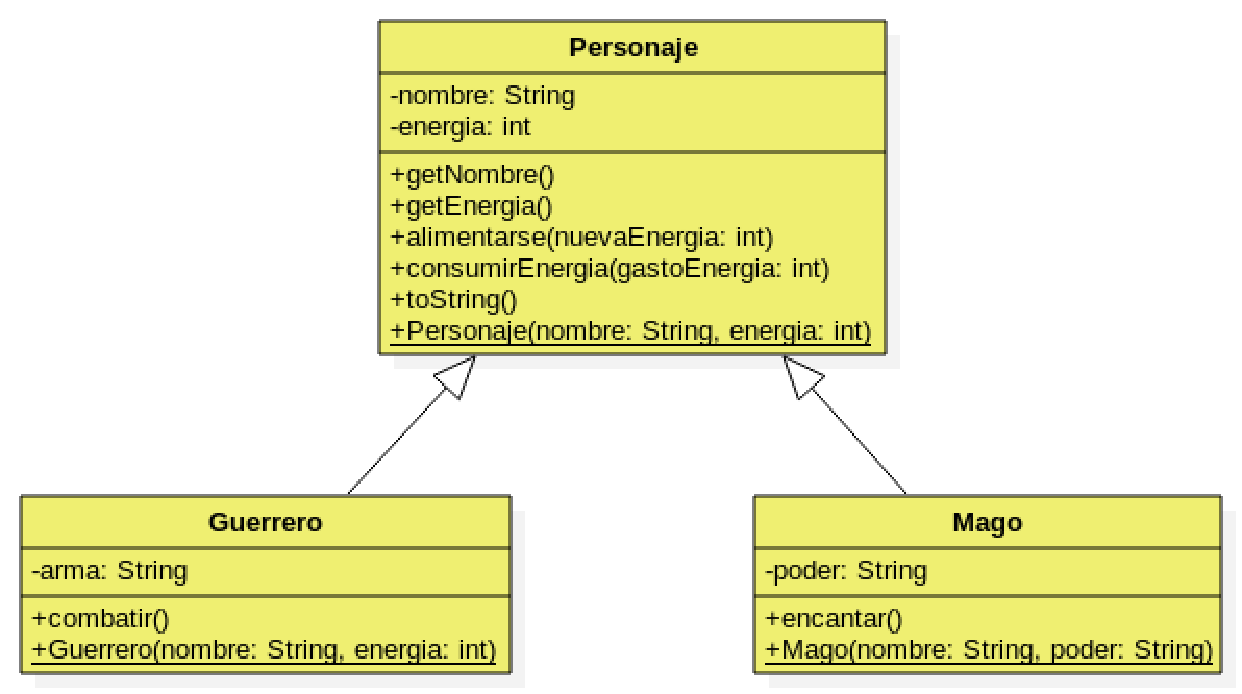
\includegraphics[width=10cm]{modelo.pdf}
				\caption{{\small Diagrama de clases}}\label{fig-modelo}
			\end{center}
		\end{figure}
		\item[] Desarrolle las clases mostradas en el modelo y la clase principal que permita instanciar personajes de tipo guerreros y magos, y utilice sus m\'etodos para \emph{combatir} y \emph{alimentarse}. Muestre en todo momento, el \emph{nivel propio de energ\'ia} que posee cada personaje.
	    \end{enumerate}
%	    \newpage
%	    \item Dentro de las figuras geom\'etricas el \textbf{Tri\'angulo}, el \textbf{Cuadril\'atero} y el \textbf{C\'irculo} son ampliamente conocidos. Es factible calcular, para cada uno de ellos, el \emph{per\'imetro} y el \emph{\'area}, siendo este c\'alculo diferente.
%	    \begin{enumerate}
%		    \item \textbf{Tri\'angulo}
%		    \begin{enumerate}
%			    \item[I.] Per\'imetro: $a + b + c$
%    			    \item[II.] \'Area: $\dfrac{bh}{2}$
%			\end{enumerate}
%			\item \textbf{Cuadril\'atero}
%		    \begin{enumerate}
%			    \item[I.] Per\'imetro: $a + b + c + d$
%    			    \item[II.] \'Area: 
%    				\begin{enumerate}
%				    \item[i.] Rect\'angulos: $ab$
%    				    \item[ii.] Cuadrados: $a^{2}$
%    				    \item[iii.] Rombo: $\dfrac{Dd}{2}$
%				\end{enumerate}
%			\end{enumerate}
%			\item \textbf{C\'irculo}
%		    \begin{enumerate}
%			    \item[I.] Per\'imetro: $2\pi r$
%    			    \item[II.] \'Area: $\pi r^{2}$
%			\end{enumerate}
%		\item[] Adem\'as, cada figura geom\'etrica tiene un \emph{tipo} que se define a partir de sus caracter\'isticas, por ejemplo, existen tri\'angulos equil\'ateros (todos sus lados iguales), is\'oceles (dos lados iguales y uno distinto) y escalenos (todos sus lados distintos). En relaci\'on a los cuadril\'ateros existen los rect\'angulos (\'angulos de $90^{\circ}$ y $2$ par lados iguales), cuadrados (\'angulos de $90^{\circ}$ y sus $4$ lados iguales), rombo (los \'angulos opuestos son iguales, distintos de $90^{\circ}$ y sus lados tambi\'en son iguales).
%		\item[] Defina la interfaz \textbf{FiguraGeometrica} que declare los m\'etodos abstractos \emph{per\'imetro}, \emph{\'area} y \emph{tipo}, para ser implementados en las clases \textbf{Triangulo}, \textbf{Cuadrilatero} y \textbf{Circulo}. Adem\'as, agregue los atributos para cada clase (grado, lado, etc) y los constructores que permitan instanciar los atributos. Finalmente, muestre toda la informaci\'on de cada figura geom\'etrica (\emph{toString}).
%		\end{enumerate}
		\newpage
		\item Un Renta Car ha solicitado un programa que permita gestionar los veh\'iculos que presta como servicio de arriendo. El Renta Car posee Autom\'oviles, Suv, Camiones y Motocicletas. La soluci\'on a plantear, debe considerar una clase padre \textbf{Veh\'iculo} con los atributos; \emph{precio}, \emph{color}, \emph{patente}, \emph{kilometraje}, \emph{octanaje} y \emph{capacidad de almacenamiento de combustible}. Adem\'as de incorporar los m\'etodos \emph{encender} y \emph{apagar}, la clase debe incluir los m\'etodos de acceso (get y set) para cada atributo. En lo que respecta a:
		 \begin{enumerate}
		    \item \textbf{Autom\'oviles}: Turbo
		    \item \textbf{Suv}: Tracci\'on (delantera$/+$trasera)
		    \item \textbf{Camiones}: Carga (en kg)
  		    \item \textbf{Motocicletas}: Cilindrada
		\end{enumerate}
		\item[] Defina las clases para cada tipo de ve\'iculos con los atributos propios y los m\'etodos de acceso (set y get). Redefina los m\'etodos \emph{encender} y \emph{apagar} de la super clase.Luego, defina la clase principal que permita instanciar al menos dos veh\'iculos por tipo (con informaci\'on ingresada desde la entrada est\'andar) y muestre toda su informaci\'on en la salida est\'andar. 
	\end{enumerate}
\end{document}